\section{Evaluation}
\label{sec:evaluation}

The evaluation addresses three research questions:
(RQ1) whether definitive answers and their evidence remain consistent with
the declared semantics as premises change;
(RQ2) what performance and completeness tradeoffs arise from bounded
reasoning, materialization, and evidence generation; and
(RQ3) which behaviors agree across native and WebAssembly execution.
It evaluates the integrated engine at revision \texttt{\EngineRevision}.
The experimental source fingerprint is \texttt{\ArtifactRevision}; the complete
file hashes, dependency locks, commands, tool versions, and machine description
are retained in the artifact.

\subsection{Protocol and comparison boundary}

Measurements run serially on the same local WSL2 machine using release builds.
The host reports an \CpuModel, with \VisibleCpus\ logical processors and
\VisibleMemoryGiB~GiB of memory visible to WSL2. The artifact records CPU
affinity, operating system, tool executable paths, and build profile.
Rust uses optimization level
3, fat link-time optimization, one code-generation unit, and abort-on-panic.
The locked paper shell includes clingo, \Souffle, Vampire, Lean, Wasmtime, Node,
and the plotting and typesetting tools. Verification and artifact compilation
finish before performance collection; other activity on the workstation is an
uncontrolled source of noise.

There are five fixed data seeds, one discarded warm-up per seed and case, and
three measured repetitions. Workload and implementation order are randomized
using a recorded seed. The policy family targets approximately 100, 1,000,
and 10,000 asserted ground facts. The actual count depends on the seeded
distribution of sanitizer and waiver records and is saved for each input.
Each workload evaluates both a supported and an unsupported finding query.
The chain family uses 4, 8, 12, 16, and 32 directed edges with one transitive
rule. Its forward and reverse queries execute in separate fresh processes so
a slow forward query cannot prevent observing the reverse result.

The bounds experiment crosses materialization on/off with depths 2, 5, 10,
and 20 on a 100-fact policy workload and both directions of an eight-edge
chain. This is a fixed diagnostic slice, not a full factorial crossing of all
dataset sizes. The evidence experiment compares fresh verdict-only and
certificate-generating sessions at each policy size. Update sequences use
approximately 100 and 1,000 facts, with both kinds of support, reassertion,
and two saved-state reopenings. The sizes and slices were frozen after harness
validation and before collection.

For the cross-system comparison, separate renderers generate KR, clingo input,
and \Souffle\ input from a common description of atoms and rules. They do not
translate another engine's emitted source. Hand-derived positive and negative
cases validate argument order, variable sharing, default negation, and support
alternatives. Predicate names are prefixed in the \Souffle\ adapter to avoid
reserved built-ins; constants are represented as opaque symbols, not integers.
The pilot exposed the reserved \texttt{cat} spelling and the final adapter
explicitly tests that translation.

The comparison unit is a complete ground-query workload: process start, full
input load, evaluation of every listed query, and output. A demand-driven
engine may compute less of a relation than an eager engine while satisfying
that same workload. Accordingly, these results are not a comparison of full
relation enumeration throughput. Nibli loads one source statement per public
\texttt{assert\_text} call, retaining the resulting source IDs. Thus loading
includes per-statement admission and state publication; this is not a bulk
ingestion throughput measurement. The baselines load their generated input
files through their ordinary command-line interfaces.
clingo is invoked with one worker and a
single stable model, sufficient for these stratified programs. \Souffle\ runs
as a compiled executable with one worker, default optimizations, and no
requested magic-set transformation. It reads external fact files, so compilation
does not precompute an answer from embedded data. Its interpreted mode is not
mixed into the comparison~\cite{souffle-execute}.

Preparation is recorded separately: neutral input translation, \Souffle\ source
generation and C++ compilation, and executable reuse keyed by generated source.
Nibli's KR parsing and semantic compilation occur inside its loading phase.
Building the generic Rust engine and installing the solver binaries are outside
the workload timings for all systems.
Compilation measurements cover \CompiledPrograms\ distinct programs, with a
median of \CompilationMedianMs~ms and interquartile endpoints
\CompilationQOneMs\ and \CompilationQThreeMs~ms. These costs should be included
when choosing a system for a one-off job. Each distinct generated program is
compiled once; these quartiles describe that set of preparations, not repeated
builds of one program. Nibli-specific loading and query
timings are useful phase diagnostics, but cannot be compared directly with
another system's whole-process latency.

\subsection{Accounting for incomplete observations}

Each execution has a 30-second external cutoff. A timeout is recorded as a
process outcome, separately from \Resource\ returned by the engine.
Standard output is flushed after each Nibli phase so completed loading and
earlier answers remain visible when a later phase is cut off. Raw output,
exit status, elapsed time, peak process resident memory, source snapshots,
and update instructions accompany the observation.

Tables report medians and linear-interpolated quartiles over the 15 measured
samples in a cell. Latency summaries use completed processes only; cutoff
counts accompany them. They do not replace a censored sample with 30 seconds
or silently omit it from the outcome ledger. Definitive-answer coverage uses
all planned answers as the denominator, so a process that times out before
answering does not improve coverage by disappearing. Repeated samples describe
this machine and these seeded inputs, not independent deployment populations;
we do not report significance tests or claim broad scaling laws.

\subsection{Definitive answers and premise changes (RQ1)}

Across the timed experiments, the ledger contains \MeasuredRuns\ measured runs
and \WarmupRuns\ warm-ups. There are \DefinitiveMismatches\ disagreements between
observed definitive answers and the workload expectations.
Appendix~\ref{app:outcomes} lists unresolved answers, resource outcomes,
process failures, and cutoffs separately. These counts qualify the agreement
claim: an absent answer is not evidence of semantic agreement.

The update sequence queries authorization and findings after every mutation.
Within measured native evidence and update runs, the audit checks
\CertificateCount\ recorded certificate envelopes and
\CitationCount\ source citations, with \CitationErrors\ source-liveness or label
errors. These are emitted certificate and citation occurrences, not counts of
independent proofs or unique premises. Table~\ref{tab:update} separates loading,
withdrawal, and reopen work. Withdrawal and reopening columns sum the operations
of that kind within one sequence; certificate and reassertion phase measurements
remain available in the CSV data.

\begin{table}[t]
\centering\small
\begin{tabular}{rlllr}
\toprule
Target facts & Load ms [Q1,Q3] & Withdrawals ms & Reopens ms & Completed \\
\midrule
100 & 367.4 [351.4, 381.0] & 7.80 [7.45, 9.03] & 622.7 [598.2, 648.0] & 15/15 \\
1000 & 7,928 [7,620, 8,184] & 309.4 [70.3, 425.1] & 14,021 [13,649, 14,814] & 14/15 \\
\bottomrule
\end{tabular}

\caption{Native persistent update sequences. Reopen means closing and opening
the database, with the profile reapplied. Timings are milliseconds; interval
endpoints are the first and third quartiles.}
\label{tab:update}
\end{table}

This evidence supports the specific transition behavior of the integrated
engine. The broader retraction differential supplies additional coverage for
domain and equality reconstruction. Neither constitutes an incremental-update
performance comparison with RDFox, clingo, or \Souffle; no equivalent baseline
update API was measured.

\subsection{Latency, bounds, and evidence (RQ2)}

\begin{table}[t]
\centering\small
\begin{tabular}{rlrrr}
\toprule
Target facts & System & Wall ms [Q1, Q3] & RSS MiB & Cutoffs \\
\midrule
100 & clingo & 4.98 [4.66, 5.42] & 7.70 & 0/15 \\
100 & Nibli & 47.0 [45.2, 48.7] & 6.29 & 0/15 \\
100 & Souffl\'e & 4.66 [4.37, 5.16] & 5.65 & 0/15 \\
1000 & clingo & 7.61 [7.17, 7.97] & 7.95 & 0/15 \\
1000 & Nibli & 3,950 [3,832, 4,057] & 22.7 & 0/15 \\
1000 & Souffl\'e & 5.28 [4.76, 5.60] & 5.77 & 0/15 \\
10000 & clingo & 30.3 [29.7, 31.0] & 10.2 & 0/15 \\
10000 & Nibli & \textit{no completion} & -- & 15/15 \\
10000 & Souffl\'e & 8.14 [7.83, 8.55] & 6.52 & 0/15 \\
\bottomrule
\end{tabular}

\caption{Complete policy workloads, including process startup and input loading.
RSS is peak resident memory for the whole process. The target size excludes
rules; exact ground-fact counts are retained per seed.}
\label{tab:policy}
\end{table}

\begin{figure}[t]
\centering
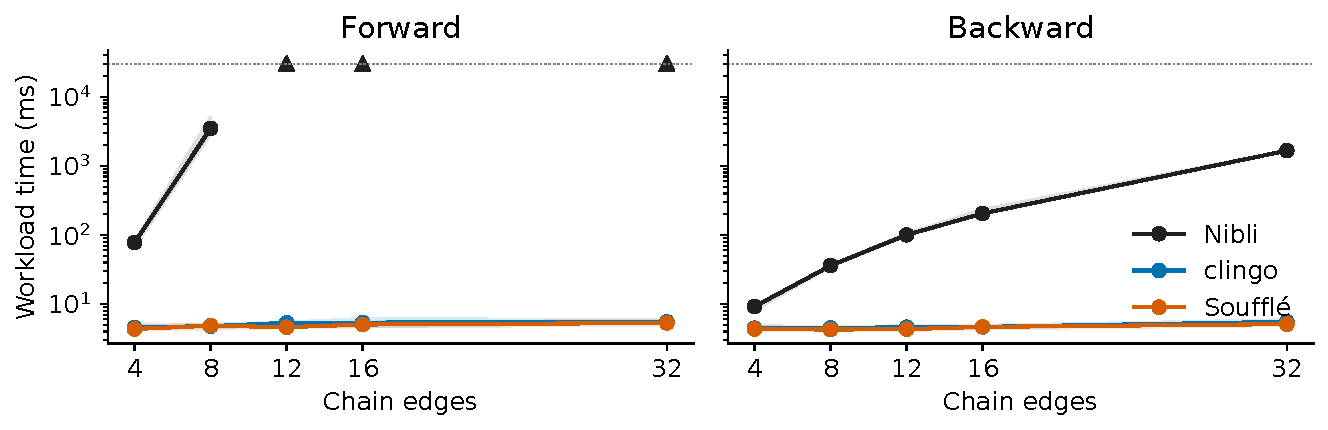
\includegraphics[width=\linewidth]{generated/reachability.pdf}
\caption{Fresh-process recursive reachability under the default comparison profile. Bands show
interquartile ranges of completed runs. Triangles at the cutoff line indicate
cells with externally timed-out runs; they are not completed latency points.}
\label{fig:reachability}
\end{figure}

Table~\ref{tab:policy} and Figure~\ref{fig:reachability} distinguish policy joins
from recursive reachability. The repository documented a severe forward-query
cost increase in an earlier measurement. Both directions and the unfavorable
sizes remain in the frozen experiment. The new data determine how much of that
behavior remains at this baseline; older timings are not copied into the results.
In particular, an empirical increase over a short chain series is not by itself
a proof of exponential asymptotic complexity.

Both comparators complete the measured policy workloads substantially faster
than Nibli where all systems finish. Nibli's loading phase dominates its
1,000-fact fresh-process cost, while the internal verdict queries take only a
small part of that time. This result characterizes the per-statement public API
workflow; it does not isolate the cost of each compiler, indexing, or state
publication mechanism.

\begin{figure}[t]
\centering
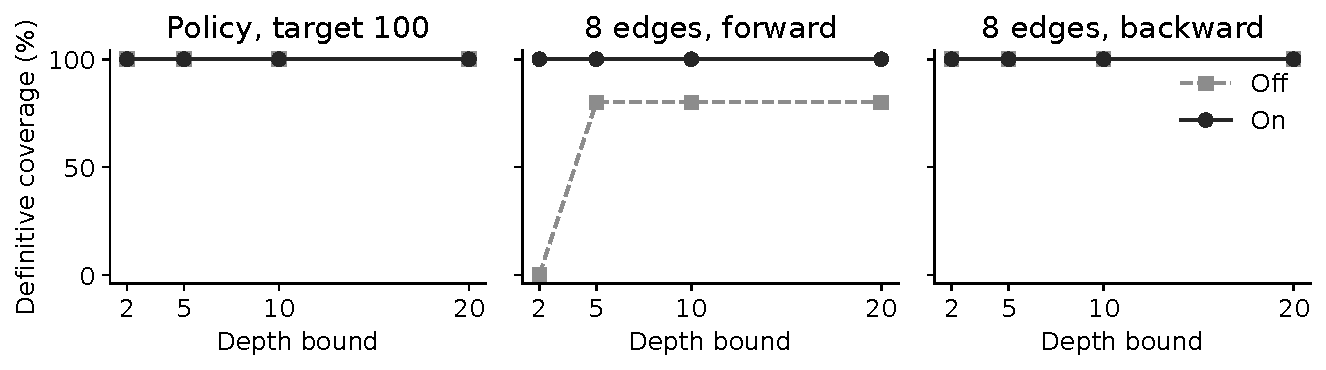
\includegraphics[width=\linewidth]{generated/bounds.pdf}
\caption{Definitive coverage in the fixed bounds slice. The denominator includes
all planned answers, including those not emitted before a process cutoff.}
\label{fig:bounds}
\end{figure}

Materialization-on and materialization-off runs give \BoundsComparable\
paired answers that are definitive in both modes, with \BoundsChanges\
definitive disagreements. A further \BoundsGains\ paired answers change from a
returned non-definitive outcome with materialization off to a definitive
outcome with it on. External timeouts are not relabeled as such returned
completeness gains. Figure~\ref{fig:bounds} reports overall coverage for each
mode and bound, which also exposes missing answers. There are
\BoundsRegressions\ paired changes in the opposite direction, from a returned
definitive answer with materialization off to a non-definitive answer with it on.
All observed gains are in the eight-edge forward workload. The unresolved
off-mode answers at larger depths carry \texttt{CycleCut}: increasing the
depth alone does not eliminate these call-path cuts, even though the input
edge chain is acyclic. Policy and reverse-chain queries are already definitive
throughout the tested bounds in both modes.

\begin{table}[t]
\centering\small
\begin{tabular}{rllrr}
\toprule
Target facts & Verdict ms [Q1,Q3] & Certificate ms [Q1,Q3] & JSON bytes & Cutoffs V; C \\
\midrule
100 & 0.345 [0.341, 0.362] & 3.25 [3.13, 3.60] & 105,191 & 0/15; 0/15 \\
1000 & 1.99 [1.88, 2.10] & 79.4 [77.9, 82.6] & 971,521 & 0/15; 0/15 \\
10000 & \textit{no completion} & \textit{no completion} & -- & 15/15; 15/15 \\
\bottomrule
\end{tabular}

\caption{Nibli evidence cost on fresh sessions. Each internal query measurement
is the sum for the two policy queries. Certificate time includes reasoning
and trace construction; validation and serialization are timed separately in
the artifact. JSON size is the sum of emitted envelope bytes. Cutoffs are
listed separately for verdict mode (V) and certificate mode (C).}
\label{tab:evidence}
\end{table}

Table~\ref{tab:evidence} measures the execution distinction described in
Section~\ref{sec:architecture}. It compares fresh sessions so the verdict-only
run cannot prewarm the traced run. The first and second queries within each
session are ordered identically in both modes. This experiment measures an
application choosing an evidence-producing API, not a constant serialization
tax added to an otherwise identical inference path.
The serialization phase times one encoding of the envelope. Constructing and
writing the full raw log adds further harness work to whole-process time;
it is outside the reported internal query and certificate timings.

% Generated from measured observations; never hand-edit numbers.
The largest policy cases expose an ingestion limit in this workflow. Of 45 measured Nibli runs at the 10,000-fact target across the comparison and evidence groups, 45 reach the external cutoff; 45 do so before loading completes. These runs provide no completed query or certificate timing. The result concerns the recorded sequence of public API calls, including admission and state publication. It does not isolate parser throughput or prove that every bulk-ingestion strategy has the same limit.

The recursive asymmetry is also substantial: forward queries on chains of 12, 16, and 32 edges reach the cutoff in 45 of 45 measured runs, while 45 of 45 reverse-query runs complete. Dataset size alone therefore gives a poor account of the cost: the requested direction and evaluation path matter. A higher depth bound is not a time budget, and an eligible finite relation does not imply that the engine will eagerly complete it before attempting a positive query.

At the 1,000-fact target, the ratio of median certificate time to median verdict-only query time is 39.9. This is a ratio of two fresh-session medians, not a paired speedup estimate. The median separately measured JSON serialization time is 0.707~ms. The distinction between evidence-producing reasoning and serialization is consequential: the former requests a trace through an execution path that retains backward derivation work. The comparison does not attribute every part of that difference to one internal optimization.


\subsection{Portable behavior and host limits (RQ3)}

The shared portability series covers policy findings, both reachability
directions, withdrawal with alternative support, generated witness separation
from an equal-looking user string, and tense discrimination. It uses the same
request snapshots for native Rust, the WASI component executed by the Wasmtime
host, and the wasm-bindgen wrapper under Node/V8. Five seeds, one warm-up,
three recorded repetitions, and randomized runtime order yield
\PortableComparisons\ measured process scenarios and \PortableAnswers\
query outcomes. There are \PortableFailures\ failed scenario comparisons.
This tests verdicts and relevant profile fields, not byte-identical proof
serialization or performance portability.

The comparison provides adequate host budgets. Fuel exhaustion and recovery
are tested separately by the host suite: a deliberately small fuel budget
produces a resource result, then raising the budget permits reconstruction,
replay, and a subsequent definitive query. Browser execution does not expose
the same fuel meter or durable database interface. Saved-state reopening is
therefore established for the persistent native and Wasmtime paths by their
respective checks, not attributed to the browser wrapper.
